\documentclass[../main/main.tex]{subfiles}

\begin{document}
\espacio
  En este capítulo se muestran los conceptos referentes a computación paralela en CPU y GPU, definición y estructura del algoritmo AES Rijndael, operaciones utilizadas para el cifrado y descifrado, muestras y resultados obtenidos de la ejecución del algoritmo AES Rijndael en CPU y GPU.

  \section{Antecedentes}

  \subsection{Computación paralela}

  La computación paralela es una rama de la informática que se encarga del estudio de la ejecución de una tarea dividida en sub-procesos o varias tareas independientes de forma simultánea en forma de hilos de ejecución en un grupo de procesadores llamados también procesadores multinúcleo, que luego de realizar dichas tareas sincronizan sus resultados a fin de mantener la integridad de los datos.

  \begin{figure}
    \centering
    \caption{Disposición de un microprocesadores multinúcleo}
    \tikzset{every picture/.style={line width=0.75pt}} %set default line width to 0.75pt        

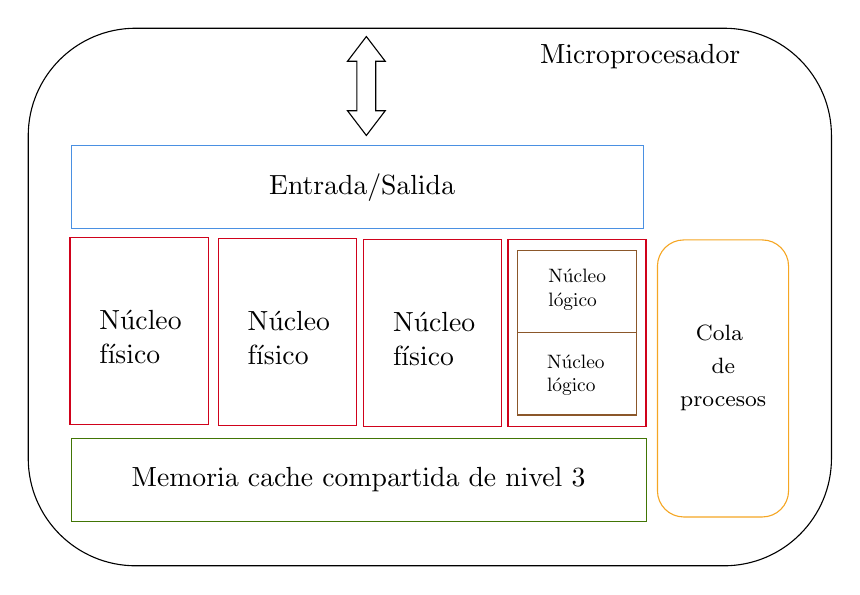
\begin{tikzpicture}[x=0.75pt,y=0.75pt,yscale=-1,xscale=1]
%uncomment if require: \path (0,300); %set diagram left start at 0, and has height of 300

%Shape: Rectangle [id:dp7451660985771589] 
\draw  [color={rgb, 255:red, 208; green, 2; blue, 27 }  ,draw opacity=1 ] (100.31,108) -- (166.81,108) -- (166.81,198.2) -- (100.31,198.2) -- cycle ;

%Shape: Rectangle [id:dp20887119442499946] 
\draw  [color={rgb, 255:red, 208; green, 2; blue, 27 }  ,draw opacity=1 ] (171.81,108.5) -- (238.31,108.5) -- (238.31,198.7) -- (171.81,198.7) -- cycle ;

%Shape: Rectangle [id:dp7286280016278224] 
\draw  [color={rgb, 255:red, 208; green, 2; blue, 27 }  ,draw opacity=1 ] (241.81,109) -- (308.31,109) -- (308.31,199.2) -- (241.81,199.2) -- cycle ;

%Shape: Rectangle [id:dp10536868660856769] 
\draw  [color={rgb, 255:red, 208; green, 2; blue, 27 }  ,draw opacity=1 ] (311.31,109) -- (377.81,109) -- (377.81,199.2) -- (311.31,199.2) -- cycle ;
%Shape: Rectangle [id:dp1826752439641639] 
\draw  [color={rgb, 255:red, 65; green, 117; blue, 5 }  ,draw opacity=1 ] (101.17,205.17) -- (378.06,205.17) -- (378.06,245.17) -- (101.17,245.17) -- cycle ;
%Rounded Rect [id:dp2234320479476144] 
\draw  [color={rgb, 255:red, 245; green, 166; blue, 35 }  ,draw opacity=1 ] (383.33,121.97) .. controls (383.33,114.99) and (388.99,109.33) .. (395.97,109.33) -- (433.87,109.33) .. controls (440.84,109.33) and (446.5,114.99) .. (446.5,121.97) -- (446.5,230.17) .. controls (446.5,237.14) and (440.84,242.8) .. (433.87,242.8) -- (395.97,242.8) .. controls (388.99,242.8) and (383.33,237.14) .. (383.33,230.17) -- cycle ;
%Shape: Rectangle [id:dp1417047542970684] 
\draw  [color={rgb, 255:red, 74; green, 144; blue, 226 }  ,draw opacity=1 ] (101,64) -- (376.5,64) -- (376.5,104) -- (101,104) -- cycle ;
%Shape: Rectangle [id:dp36104680527645483] 
\draw  [color={rgb, 255:red, 139; green, 87; blue, 42 }  ,draw opacity=1 ] (316,114.5) -- (373.25,114.5) -- (373.25,154.1) -- (316,154.1) -- cycle ;
%Shape: Rectangle [id:dp8737201655413631] 
\draw  [color={rgb, 255:red, 139; green, 87; blue, 42 }  ,draw opacity=1 ] (316,154.1) -- (373.25,154.1) -- (373.25,193.7) -- (316,193.7) -- cycle ;
%Rounded Rect [id:dp23562455979240182] 
\draw   (80.17,59.13) .. controls (80.17,30.52) and (103.36,7.33) .. (131.97,7.33) -- (415.37,7.33) .. controls (443.98,7.33) and (467.17,30.52) .. (467.17,59.13) -- (467.17,214.53) .. controls (467.17,243.14) and (443.98,266.33) .. (415.37,266.33) -- (131.97,266.33) .. controls (103.36,266.33) and (80.17,243.14) .. (80.17,214.53) -- cycle ;
%Up Down Arrow [id:dp8508564601094952] 
\draw   (234,23.25) -- (243.08,11.33) -- (252.17,23.25) -- (247.62,23.25) -- (247.62,47.08) -- (252.17,47.08) -- (243.08,59) -- (234,47.08) -- (238.54,47.08) -- (238.54,23.25) -- cycle ;

% Text Node
\draw (134.25,156) node  [align=left] {Núcleo\\ físico};
% Text Node
\draw (205.75,156.5) node  [align=left] {Núcleo\\ físico};
% Text Node
\draw (275.75,157) node  [align=left] {Núcleo\\ físico};
% Text Node
\draw (239.33,224.67) node  [align=left] {Memoria cache compartida de nivel 3};
% Text Node
\draw (415,171) node  [align=left] {{\footnotesize  \ \ Cola}\\{\footnotesize  \ \ \ \ de}\\{\footnotesize procesos}};
% Text Node
\draw (241,84) node  [align=left] {Entrada/Salida};
% Text Node
\draw (344.67,133.33) node [scale=0.7] [align=left] {Núcleo\\ lógico};
% Text Node
\draw (344,174.33) node [scale=0.7] [align=left] {Núcleo\\ lógico};
% Text Node
\draw (375,21) node  [align=left] {Microprocesador};


\end{tikzpicture}
    \caption*{\textbf{Fuente:} Elaboración propia}
  \end{figure}

  Los microprocesadores actuales contienen comúnmente dos tipos de núcleos, los núcleos físicos y los núcleos lógicos. Cada zócalo de una tarjeta madre contiene un microprocesador, este contiene uno o más núcleos físicos; un núcleo físico es aquel que se encuentra físicamente dentro del circuito integrado del microprocesador, mientras que un núcleo lógico es una división virtual en 2 o más partes de un núcleo físico. Las tareas son asignadas a los núcleos físicos; estas tareas pueden dividirse en tareas más pequeñas a fin de resolver un gran problema en partes pequeñas que al final serán unidas para generar la solución, estas partes pequeñas son llamadas ``hilos'' y son las que se ejecutan en los núcleo lógicos.

  \textit{Las técnicas principales para lograr estas mejoras de rendimiento (mayor frecuencia de reloj y arquitecturas cada vez más inteligentes y complejas) están golpeando la llamada ``Power Wall''. La industria informática ha aceptado que los futuros aumentos en rendimiento deben provenir en gran parte del incremento del número de procesadores (o núcleos) en una matriz, en vez de hacer más rápido un solo núcleo.} [\cite[p.~6]{report:parallel_computing_illinois}]

  El incremento de la frecuencia en los microprocesador acarrea consigo el consumo de energía y la disminución del espacio entre los transistores dentro de cada núcleo, lo que provoca un incremento considerable de la temperatura dentro del microprocesador; por tanto, para mantener el microprocesador en funcionamiento evitando su deterioro por las temperaturas elevadas es necesario buscar fuentes más óptimas de enfriado como los tubos de conducción de gas o líquido, que incrementan aún más el consumo de energía y que son costosos para una PC de escritorio.

  \vspace{-0.7cm}\begin{equation}
    T_m = T_a \cdot [( 1 - F_m ) + \frac{F_m}{A_m}]
    \label{ecuacion_amdahl}
  \end{equation}

  Donde:

  \begin{description}[noitemsep, nolistsep]
    \item[$F_m=$] Fracción de tiempo que el sistema utiliza el subsistema mejorado
    \item[$A_m=$] Factor de mejora que se ha introducido en el subsistema mejorado
    \item[$T_a=$] Tiempo de ejecución antiguo
    \item[$T_m=$] Tiempo de ejecución mejorado
  \end{description}

  Por tales motivos Gene Amdahl formuló la ecuación \ref{ecuacion_amdahl} que establece que:

  \textit{La mejora obtenida en el rendimiento de un sistema debido a la alteración de uno de sus componentes está limitada por la fracción de tiempo que se utiliza dicho componente}

  Despejando la ecuación \ref{ecuacion_amdahl} se obtiene la aceleración del programa completo una vez que se haya paralelizado uno o más algoritmos del programa.

  \vspace{-0.7cm}\begin{equation}
    A = \frac{1}{( 1 - F_m ) + \frac{F_m}{A_m}}
    \label{ecuacion_amdahl_aceleracion}
  \end{equation}

  Donde:

  \begin{description}[noitemsep, nolistsep]
    \item[$A=$] Aceleración o ganancia en velocidad conseguida en el sistema completo debido a la mejora de uno de sus subsistemas
    \item[$A_m=$] Factor de mejora que se ha introducido en el subsistema mejorado
    \item[$F_m=$] Fracción de tiempo que el sistema utiliza el subsistema mejorado
  \end{description}

  \begin{figure}[H]
    \centering
    \caption{Clúster de alto rendimiento}
    \includegraphics[width=8cm, keepaspectratio]{marco_teorico/cluster_alto_rendimiento.jpg}
    \caption*{\textbf{Fuente:} \cite[p.~2]{article:cluster_alto_rendimiento}}
  \end{figure}

  En base a este principio se desarrollaron tecnologías de matrices de núcleos de cómputo tomando como elementos principales a los procesadores existentes y acomodándolos de tal forma que se pueda administrar la ejecución de tareas en cada procesador de manera individual y la sincronización de resultados al final del proceso. Estos arreglos reciben el nombre de clústers. Los clústers de alto rendimiento son un tipo de clústers utilizados con el propósito de ejecutar tareas exhaustivas divididas en tareas pequeñas ejecutadas en cada computador de acuerdo a la gestión realizada por el llamado nodo maestro. [\cite{article:cluster_alto_rendimiento}]

  \begin{figure}[H]
    \centering
    \caption{Comparación de tiempos de proceso en múltiples CPUs}
    \includegraphics[width=15cm, keepaspectratio]{marco_teorico/resultado_cpu_cluster.png}
    \caption*{\textbf{Fuente:} \cite[p.~7]{article:cluster_alto_rendimiento}}
  \end{figure}

  \subsection{Unidad de procesamiento gráfico (GPU)}

  Esta unidad actúa como un co-procesador que se encarga de las operaciones matriciales o de coma flotante, por lo general los procesos gráficos de transformación o renderización son distribuidos a la o las GPUs desde el procesador central o CPU.

  Dado el estudio generado sobre las plataformas GPU, los fabricantes pusieron a disposición de los usuarios herramientas de desarrollo para utilizar las GPU como ayuda en cálculos de álgebra dispersa, tensores en dinámica de fluidos, minería de datos, inteligencia artificial, deep learning, etc, con lo cual la denominación de las GPU abiertas a otro tipo de uso más que el simple uso gráfico cambió a GPGPU\footnote{Unidad de Procesamiento Gráfico de Uso General (General Purpose Graphics Processing Unit)}.

  Estas tarjetas están desarrolladas en base al paralelismo de núcleos de frecuencia baja con un esquema de operaciones limitado.

  \begin{figure}[H]
    \centering
    \caption{Cantidad de núcleos en CPU vs GPU}
    \includegraphics[width=15cm, keepaspectratio]{marco_teorico/cpu_vs_gpu_cores.jpg}
    \caption*{\textbf{Fuente:} \cite{web:gpgpu}}
  \end{figure}

  El obstáculo principal para el desarrollo de aplicaciones orientadas hacia la GPU es que las arquitecturas de las tarjetas gráficas son demasiado variables, a pesar de la existencia de librerías o APIs genéricas como OpenGL, muchas funcionalidades dentro de los métodos o clases son variables entre fabricantes e incluso entre modelos de dispositivos de un mismo fabricante. Las librerías genéricas utilizan un núcleo basado en el esquema de Conductos de Renderización\footnote{Rendering Pipeline}, con los que se pueden tratar vectores, mapas de bits y elementos definidos pixel-pixel.

  Otro factor importante que impide hacer un uso adecuado de estos dispositivos es el límite físico con el que actualmente cuenta la conexión de memoria RAM de la GPU con el bus de la CPU para la transferencia de datos. Al cuarto trimestre de 2018 ya se cuenta con la tecnología GDDR6\footnote{Tasa Doble de transferencia de Datos  (Double Data Rate)} que ofrece un ancho de banda de hasta 16Gbps frente a los 10Gbps de su predecesor GDDR5X, cabe mencionar que se lograron estos anchos de banda gracias al cambio de modo half-duplex o transferencia en ambos sentidos pero solo uno a la vez, por el modo full-duplex que transfiere los datos en ambos sentidos al mismo tiempo.

  \begin{figure}[H]
    \centering
    \caption{Comparación de tecnologías GDDR6 vs GDDR5}
    \includegraphics[width=12cm, keepaspectratio]{marco_teorico/comparacion_gddr.png}
    \caption*{\textbf{Fuente:} \cite{web:comparacion_gddr}}
  \end{figure}

  Pero AMD ya se encuentra desarrollando tarjetas madres con conectores PCI-E\footnote{Componente Periférico de Interconexión Expresa (Peripheral Component Interconnect Express)} 5.0 que incrementarán la velocidad de transferencia hasta los 32Gbps que conjuntamente con el almacenamiento SSD\footnote{Solid State Drive} lograrán impulsar el desarrollo de aplicaciones de uso general en las GPUs.

  \begin{table}[H]
    \centering
    \caption{Comparación de tecnologías PCI-E}
    \begin{tabular}{c|c|c|c|c|}
  \cline{2-5}
                                          & \textbf{RAW Bitrate} & \textbf{Link BW} & \textbf{BW/Lane/Way} & \textbf{Total BW X16} \\ \hline
  \multicolumn{1}{|c|}{\textbf{PCIe 1.x}} & 2.5 GT/s             & 2 Gb/s           & 250 MB/s             & 8 GB/s                \\ \hline
  \multicolumn{1}{|c|}{\textbf{PCIe 2.x}} & 5.0 GT/s             & 4 Gb/s           & 500 MB/s             & 16 GB/s               \\ \hline
  \multicolumn{1}{|c|}{\textbf{PCIe 3.x}} & 8.0 GT/s             & 8 Gb/s           & $\sim$1 GB/s         & $\sim$32 GB/s         \\ \hline
  \multicolumn{1}{|c|}{\textbf{PCIe 4.x}} & 16 GT/s              & 16 Gb/s          & $\sim$2 GB/s         & $\sim$64 GB/s         \\ \hline
  \multicolumn{1}{|c|}{\textbf{PCIe 5.x}} & 32 GT/s              & 32 Gb/s          & $\sim$4 GB/s         & $\sim$128 GB/s        \\ \hline
  \end{tabular}
    \caption*{\textbf{Fuente:} \cite{web:comparacion_pcie}}
  \end{table}

  \section{Algoritmo Estándar de Encriptación Avanzada Rijndael}

  El Estándar de Encriptación Avanzada fue de desarrollado mediante un concurso en 1997, por los criptógrafos Vincent Rijmen e Joan Daemen en el año 2001, como la sustitución al algoritmo DES\footnote{Estándar de Encriptación de Datos(Data Encryption Standard)} que había sido crackeado mediante la máquina DES Cracker construida por la ONG Electronic Frontier Foundation, con una inversión de 250 mil dólares. Este estándar fue aprobado y es utilizado por entes reguladores como la NSA\footnote{Agencia de Seguridad Nacional(National Security Agency)} y se estandariza mediante la norma ISO/IEC 18033 [\cite{standard:iso_18033}].

  El algoritmo AES Rijndael es un algoritmo de llave simétrica, lo cual indica que se utiliza una misma llave para cifrar y descifrar los mensajes en el lado del emisor y del receptor. Por tal razón, toda la seguridad recae en proteger la clave secreta, por tal razón el abanico de claves posibles debe ser de una cantidad tan grande que el intruso deba realizar pruebas, por inclusive años, para poder descifrar el mensaje. Para el caso de DES, la clave es de 56 bits por lo que la cantidad de claves será igual a: $2^{56} = 7.2 \times 10^{16}$ posibles claves; un computador actual puede lograr descifrar un mensaje mediante el cálculo de la llave secreta en un tiempo de tan solo segundos.

  \begin{table}[H]
    \centering
    \caption{Comparación de tecnologías PCI-E}
    \begin{tabular}{|c|c|}
  \hline
  \multicolumn{1}{|l|}{\textbf{Tamaño de Clave}} & \multicolumn{1}{l|}{\textbf{Combinaciones Posibles}} \\ \hline
  1 bit & $2$ \\ \hline
  2 bit & $4$ \\ \hline
  4 bit & $16$ \\ \hline
  8 bit & $256$ \\ \hline
  16 bit & $65536$ \\ \hline
  32 bit & $4.2\times10^{9}$ \\ \hline
  56 bit (DES) & $7.2\times10^{16}$ \\ \hline
  64 bit & $1.8\times10^{19}$ \\ \hline
  128 bit (AES) & $3.4\times10^{38}$ \\ \hline
  192 bit (AES) & $6.2\times10^{57}$ \\ \hline
  256 bit (AES) & $1.1\times10^{77}$ \\ \hline
  \end{tabular}
    \caption*{\textbf{Fuente:} \cite{web:tiempo_crack_aes}}
  \end{table}

  El algoritmo AES Rijndael trabaja con mensajes divididos en bloques de 128 bits y llaves de logitud de 128, 192 y 256 bits. Por lo tanto con una llave de 128 bits el atacante necesitaría generar: $2^{56} = 3.4 \times 10^{38}$ llaves, tarea que en la actualidad, aún con computadoras tan potentes, el trabajo tardaría millones de años.

  Suponiendo la super-computadora Summit de IBM [\cite{web:supercomputadora_summit_ibm}], designada para descifrar un mensaje, trabajando a $143.5PFlops$\footnote{Operaciones de Punto Flotante por Segundo(Floating point Operations Per Second)} o $143.5 \times 10^{15} Flops$ y sabiendo que la cantidad de segundos en un año es de: $365 \times 24 \times 60 \times 60 = 31536000$. Se calcula la cantidad de años necesarios para crackear AES con una longitud de clave de 128 bits.

  \vspace{-0.7cm}\begin{equation}
    \begin{aligned}
    t &= \frac{3.4 \times 10^{38}}{143.5 \times 10^{15} \times 31536000} \\
    \\
    t &= \frac{23.69 \times 10^{15}}{315.36} \\
    \\
    t &= 75.13 \times 10^{12} a\tilde{n}os
    \end{aligned}
  \end{equation}

  Es decir, con la última tecnología disponible actualmente se tomaría un tiempo de 75.13 billones de años en generar las llaves secretas necesarias para descifrar un mensaje. Suponiendo que solo fuese necesario generar la mitad de las llaves para encontrar la correcta, el proceso tardaría mas de 32 billones de años. Por lo tanto una llave secreta de 128 bits utilizada para cifrar un mensaje con el algoritmo AES Rijndael es suficiente seguridad para la actualidad y para unos años más en el futuro.

  Este algoritmo fue seleccionado ganador de entre muchos otros participantes del concurso de 1997 considerando sus tres axiomas importantes:

  \begin{itemize}[noitemsep,nolistsep]
    \item Resistencia contra todos los ataques conocidos hasta la fecha.
    \item Compatibilidad con un gran número de plataformas de hardware.
    \item Velocidad y sencillez en el diseño.
  \end{itemize}

  \subsection{Estructura del algoritmo}

    Los cifradores simétricos están desarrollados con una estructura de tipo Feistel, esta estructura tiene dos partes, la izquierda y la derecha.

    \begin{figure}[H]
      \centering
      \caption{Bloque de información H para el modelo de cifrador Feistel}
      \tikzset{every picture/.style={line width=0.75pt}} %set default line width to 0.75pt        

\begin{tikzpicture}[x=0.75pt,y=0.75pt,yscale=-1,xscale=1]
%uncomment if require: \path (0,607.4630661010742); %set diagram left start at 0, and has height of 607.4630661010742

%Shape: Rectangle [id:dp9387047590057875] 
\draw   (124,32.2) -- (159.3,32.2) -- (159.3,66.2) -- (124,66.2) -- cycle ;
%Shape: Rectangle [id:dp06134354038145262] 
\draw   (278,34.2) -- (313.3,34.2) -- (313.3,68.2) -- (278,68.2) -- cycle ;
%Straight Lines [id:da10790130820156896] 
\draw    (143,66.5) -- (143,165.5) ;


%Flowchart: Or [id:dp07980698217083693] 
\draw   (135.5,172.5) .. controls (135.5,168.63) and (138.86,165.5) .. (143,165.5) .. controls (147.14,165.5) and (150.5,168.63) .. (150.5,172.5) .. controls (150.5,176.37) and (147.14,179.5) .. (143,179.5) .. controls (138.86,179.5) and (135.5,176.37) .. (135.5,172.5) -- cycle ; \draw   (135.5,172.5) -- (150.5,172.5) ; \draw   (143,165.5) -- (143,179.5) ;
%Shape: Rectangle [id:dp9005647886302468] 
\draw   (174,155.2) -- (274,155.2) -- (274,189.2) -- (174,189.2) -- cycle ;

%Shape: Rectangle [id:dp1446172377376469] 
\draw   (128,287.2) -- (163.3,287.2) -- (163.3,321.2) -- (128,321.2) -- cycle ;
%Shape: Rectangle [id:dp5944788483468033] 
\draw   (283,288.2) -- (318.3,288.2) -- (318.3,322.2) -- (283,322.2) -- cycle ;
%Straight Lines [id:da5126430845478047] 
\draw    (297,68.5) -- (297,220) ;


%Straight Lines [id:da8558270544869495] 
\draw    (143,179.5) -- (143,221) ;


%Straight Lines [id:da15557753762708693] 
\draw    (143,221) -- (297.33,287.54) ;
\draw [shift={(299.17,288.33)}, rotate = 203.32] [color={rgb, 255:red, 0; green, 0; blue, 0 }  ][line width=0.75]    (10.93,-3.29) .. controls (6.95,-1.4) and (3.31,-0.3) .. (0,0) .. controls (3.31,0.3) and (6.95,1.4) .. (10.93,3.29)   ;

%Straight Lines [id:da21080378203535233] 
\draw    (297,220) -- (145,286.53) ;
\draw [shift={(143.17,287.33)}, rotate = 336.36] [color={rgb, 255:red, 0; green, 0; blue, 0 }  ][line width=0.75]    (10.93,-3.29) .. controls (6.95,-1.4) and (3.31,-0.3) .. (0,0) .. controls (3.31,0.3) and (6.95,1.4) .. (10.93,3.29)   ;

%Straight Lines [id:da7320888588354941] 
\draw    (228.17,119.33) -- (228.17,154.33) ;
\draw [shift={(228.17,156.33)}, rotate = 270] [color={rgb, 255:red, 0; green, 0; blue, 0 }  ][line width=0.75]    (10.93,-3.29) .. controls (6.95,-1.4) and (3.31,-0.3) .. (0,0) .. controls (3.31,0.3) and (6.95,1.4) .. (10.93,3.29)   ;

%Straight Lines [id:da6084690526516647] 
\draw    (228.17,119.33) -- (297,120) ;


%Straight Lines [id:da29161126742281174] 
\draw [color={rgb, 255:red, 255; green, 61; blue, 61 }  ,draw opacity=1 ] [dash pattern={on 4.5pt off 4.5pt}]  (326.17,172.33) -- (276.17,171.37) ;
\draw [shift={(274.17,171.33)}, rotate = 361.1] [color={rgb, 255:red, 255; green, 61; blue, 61 }  ,draw opacity=1 ][line width=0.75]    (10.93,-3.29) .. controls (6.95,-1.4) and (3.31,-0.3) .. (0,0) .. controls (3.31,0.3) and (6.95,1.4) .. (10.93,3.29)   ;

%Straight Lines [id:da9288138682659981] 
\draw    (174.17,172.33) -- (152.5,172.49) ;
\draw [shift={(150.5,172.5)}, rotate = 359.6] [color={rgb, 255:red, 0; green, 0; blue, 0 }  ][line width=0.75]    (10.93,-3.29) .. controls (6.95,-1.4) and (3.31,-0.3) .. (0,0) .. controls (3.31,0.3) and (6.95,1.4) .. (10.93,3.29)   ;


% Text Node
\draw (143,50) node  [align=left] {$\displaystyle L_{0}$};
% Text Node
\draw (297,52) node  [align=left] {$\displaystyle R_{0}$};
% Text Node
\draw (223,173) node  [align=left] {$\displaystyle Función\ F$};
% Text Node
\draw (147,305) node  [align=left] {$\displaystyle L_{1}$};
% Text Node
\draw (302,306) node  [align=left] {$\displaystyle R_{1}$};
% Text Node
\draw (339,172) node  [align=left] {$\displaystyle k_{i}$};
% Text Node
\draw (107,48) node  [align=left] {H/2};
% Text Node
\draw (331,50) node  [align=left] {H/2};


\end{tikzpicture}
      \caption*{\textbf{Fuente:} \cite{report:seguridad_europea_eeuu}}
    \end{figure}

    La diferencia es que Rijndael define las vueltas de transformaciones en tres funciones invertibles llamadas capas:

    \begin{itemize}[noitemsep,nolistsep]
      \item La mezcla lineal garantiza alta difusión de la información dado el número de vueltas.
      \item La capa no lineal hace que el comportamiento del sistema no pueda ser representado como la suma de los comportamientos de sus sub-sistemas.
      \item La capa de adición de clave crea estados intermedios para hacer difusa la matriz de estado.
    \end{itemize}

    Este algoritmo es conformado por rondas en las que se ejecutan 4 funciones matemáticas en un orden establecido. El resultado de cada ronda es llamado \textit{Estado} que es una matriz de 4 filas por $N_b$ columnas, donde:

    \vspace{-0.7cm}\begin{equation}
      N_b = \frac{Tama\tilde{n}o\ de\ bloque\ utilizado\ en\ bits}{32}
    \end{equation}

    De manera similar, la clave inicial se representa mediante una matriz de 4 filas y $N_k$ columnas, donde:

    \vspace{-0.7cm}\begin{equation}
      N_k = \frac{Tama\tilde{n}o\ de\ la\ clave\ en\ bits}{32}
    \end{equation}
    
    Las matrices se acomodan de tal forma que cada palabra (4 bytes = 32 bits) es representada en una columna de izquierda a derecha.

    Por ejemplo la frase: ``mensaje secreto.'' se convierte de ASCII a su representación hexadecimal, cuyo resultado es:

    \begin{center}
      6d 65 6e 73 61 6a 65 20 73 65 63 72 65 74 6f 2e
    \end{center}

    Que se acomoda en una matriz de estado como se muestra a continuación:

    \begin{table}[H]
      \centering
      \begin{tabular}{|l|l|l|l|}
  \hline
  6d & 61 & 73 & 65 \\ \hline
  65 & 6a & 65 & 74 \\ \hline
  6e & 65 & 63 & 6f \\ \hline
  \multicolumn{1}{|c|}{73} & 20 & 72 & 2e \\ \hline
\end{tabular}
    \end{table}

    Cabe recalcar que el mensaje es de una longitud de 128 bits; en caso de no ser así, el mensaje es dividido en paquetes de 128 bits y se acomoda un relleno o padding de acuerdo a la norma PKCS\#7 en el caso de AES Rijndael.

    De forma análoga, se realiza el mismo proceso para la clave secreta inicial que puede ser de 128, 192 o 256 bits. El número de rondas para llegar a calcular el criptograma varía de acuerdo al tamaño de la clave:

    \begin{itemize}[noitemsep,nolistsep]
      \item Para una clave de cifrado de 128 bits el algoritmo realiza 10 rondas
      \item Para una clave de cifrado de 192 bits el algoritmo realiza 12 rondas
      \item Para una clave de cifrado de 256 bits el algoritmo realiza 14 ronda
    \end{itemize}

    \subsubsection{Operaciones para el proceso de cifrado}

      \begin{figure}[H]
        \centering
        \caption{Algoritmo AES Rijndael}
        \tikzset{every picture/.style={line width=0.75pt}} %set default line width to 0.75pt        

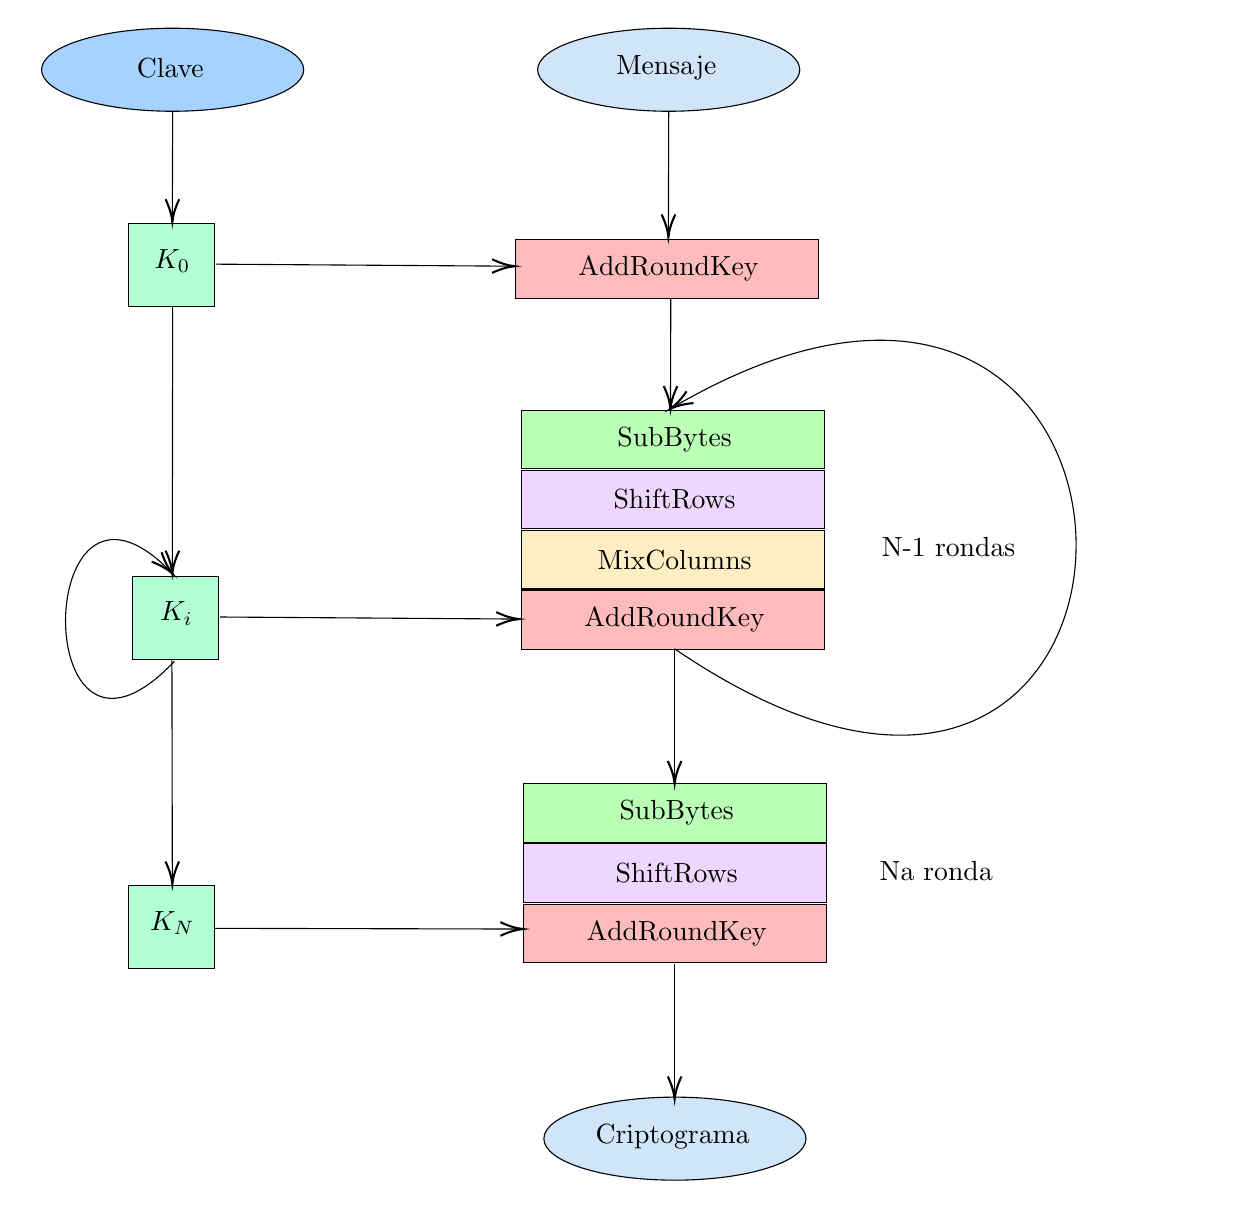
\begin{tikzpicture}[x=0.75pt,y=0.75pt,yscale=-1,xscale=1]
%uncomment if require: \path (0,607.4630661010742); %set diagram left start at 0, and has height of 607.4630661010742

%Shape: Ellipse [id:dp9737685907668199] 
\draw  [color={rgb, 255:red, 0; green, 0; blue, 0 }  ,draw opacity=1 ][fill={rgb, 255:red, 165; green, 210; blue, 255 }  ,fill opacity=1 ] (104,40) .. controls (104,28.95) and (132.27,20) .. (167.15,20) .. controls (202.03,20) and (230.3,28.95) .. (230.3,40) .. controls (230.3,51.05) and (202.03,60) .. (167.15,60) .. controls (132.27,60) and (104,51.05) .. (104,40) -- cycle ;

%Shape: Ellipse [id:dp45013119054902284] 
\draw  [color={rgb, 255:red, 0; green, 0; blue, 0 }  ,draw opacity=1 ][fill={rgb, 255:red, 208; green, 229; blue, 249 }  ,fill opacity=1 ] (343,40) .. controls (343,28.95) and (371.27,20) .. (406.15,20) .. controls (441.03,20) and (469.3,28.95) .. (469.3,40) .. controls (469.3,51.05) and (441.03,60) .. (406.15,60) .. controls (371.27,60) and (343,51.05) .. (343,40) -- cycle ;

%Shape: Rectangle [id:dp657856114899342] 
\draw  [fill={rgb, 255:red, 178; green, 255; blue, 211 }  ,fill opacity=1 ] (146,114) -- (187.3,114) -- (187.3,154) -- (146,154) -- cycle ;

%Shape: Rectangle [id:dp261406348143415] 
\draw  [fill={rgb, 255:red, 178; green, 255; blue, 211 }  ,fill opacity=1 ] (148,284) -- (189.3,284) -- (189.3,324) -- (148,324) -- cycle ;

%Shape: Rectangle [id:dp9188720632833878] 
\draw  [fill={rgb, 255:red, 178; green, 255; blue, 211 }  ,fill opacity=1 ] (146,433) -- (187.3,433) -- (187.3,473) -- (146,473) -- cycle ;

%Shape: Rectangle [id:dp25111749195065625] 
\draw  [fill={rgb, 255:red, 254; green, 187; blue, 187 }  ,fill opacity=1 ] (332.3,122) -- (478.3,122) -- (478.3,150.2) -- (332.3,150.2) -- cycle ;

%Shape: Rectangle [id:dp9024991354173098] 
\draw  [fill={rgb, 255:red, 187; green, 255; blue, 182 }  ,fill opacity=1 ] (335.3,204) -- (481.3,204) -- (481.3,232.2) -- (335.3,232.2) -- cycle ;

%Shape: Rectangle [id:dp6677044127286271] 
\draw  [fill={rgb, 255:red, 238; green, 214; blue, 255 }  ,fill opacity=1 ] (335.3,233) -- (481.3,233) -- (481.3,261.2) -- (335.3,261.2) -- cycle ;

%Shape: Rectangle [id:dp5668522361712407] 
\draw  [fill={rgb, 255:red, 255; green, 237; blue, 195 }  ,fill opacity=1 ] (335.3,262) -- (481.3,262) -- (481.3,290.2) -- (335.3,290.2) -- cycle ;

%Shape: Rectangle [id:dp34737624535273803] 
\draw  [fill={rgb, 255:red, 254; green, 187; blue, 187 }  ,fill opacity=1 ] (335.3,291) -- (481.3,291) -- (481.3,319.2) -- (335.3,319.2) -- cycle ;

%Shape: Rectangle [id:dp4367963290792771] 
\draw  [fill={rgb, 255:red, 187; green, 255; blue, 182 }  ,fill opacity=1 ] (336.3,384) -- (482.3,384) -- (482.3,412.2) -- (336.3,412.2) -- cycle ;

%Shape: Rectangle [id:dp012716397520244005] 
\draw  [fill={rgb, 255:red, 238; green, 214; blue, 255 }  ,fill opacity=1 ] (336.3,413) -- (482.3,413) -- (482.3,441.2) -- (336.3,441.2) -- cycle ;

%Shape: Rectangle [id:dp1945157717160817] 
\draw  [fill={rgb, 255:red, 254; green, 187; blue, 187 }  ,fill opacity=1 ] (336.3,442) -- (482.3,442) -- (482.3,470.2) -- (336.3,470.2) -- cycle ;

%Shape: Ellipse [id:dp0074509944076393] 
\draw  [color={rgb, 255:red, 0; green, 0; blue, 0 }  ,draw opacity=1 ][fill={rgb, 255:red, 208; green, 229; blue, 249 }  ,fill opacity=1 ] (346,555) .. controls (346,543.95) and (374.27,535) .. (409.15,535) .. controls (444.03,535) and (472.3,543.95) .. (472.3,555) .. controls (472.3,566.05) and (444.03,575) .. (409.15,575) .. controls (374.27,575) and (346,566.05) .. (346,555) -- cycle ;

%Straight Lines [id:da2019009163904124] 
\draw    (167.15,60) -- (167.01,111.33) ;
\draw [shift={(167,113.33)}, rotate = 270.15999999999997] [color={rgb, 255:red, 0; green, 0; blue, 0 }  ][line width=0.75]    (10.93,-3.29) .. controls (6.95,-1.4) and (3.31,-0.3) .. (0,0) .. controls (3.31,0.3) and (6.95,1.4) .. (10.93,3.29)   ;

%Straight Lines [id:da7298574790525367] 
\draw    (406.15,60) -- (406,118.67) ;
\draw [shift={(406,120.67)}, rotate = 270.14] [color={rgb, 255:red, 0; green, 0; blue, 0 }  ][line width=0.75]    (10.93,-3.29) .. controls (6.95,-1.4) and (3.31,-0.3) .. (0,0) .. controls (3.31,0.3) and (6.95,1.4) .. (10.93,3.29)   ;

%Straight Lines [id:da12255807726786161] 
\draw    (188,133.67) -- (330,134.65) ;
\draw [shift={(332,134.67)}, rotate = 180.4] [color={rgb, 255:red, 0; green, 0; blue, 0 }  ][line width=0.75]    (10.93,-3.29) .. controls (6.95,-1.4) and (3.31,-0.3) .. (0,0) .. controls (3.31,0.3) and (6.95,1.4) .. (10.93,3.29)   ;

%Straight Lines [id:da15131688097810092] 
\draw    (407.15,150) -- (407.01,201.33) ;
\draw [shift={(407,203.33)}, rotate = 270.15999999999997] [color={rgb, 255:red, 0; green, 0; blue, 0 }  ][line width=0.75]    (10.93,-3.29) .. controls (6.95,-1.4) and (3.31,-0.3) .. (0,0) .. controls (3.31,0.3) and (6.95,1.4) .. (10.93,3.29)   ;

%Straight Lines [id:da5876036775611393] 
\draw    (190,303.67) -- (332,304.65) ;
\draw [shift={(334,304.67)}, rotate = 180.4] [color={rgb, 255:red, 0; green, 0; blue, 0 }  ][line width=0.75]    (10.93,-3.29) .. controls (6.95,-1.4) and (3.31,-0.3) .. (0,0) .. controls (3.31,0.3) and (6.95,1.4) .. (10.93,3.29)   ;

%Straight Lines [id:da031674005498631086] 
\draw    (167.15,154) -- (167,280.67) ;
\draw [shift={(167,282.67)}, rotate = 270.07] [color={rgb, 255:red, 0; green, 0; blue, 0 }  ][line width=0.75]    (10.93,-3.29) .. controls (6.95,-1.4) and (3.31,-0.3) .. (0,0) .. controls (3.31,0.3) and (6.95,1.4) .. (10.93,3.29)   ;

%Curve Lines [id:da11017760368079688] 
\draw    (409,319) .. controls (666.24,494.29) and (668.24,49.29) .. (407,203.33) ;
\draw [shift={(407,203.33)}, rotate = 329.47] [color={rgb, 255:red, 0; green, 0; blue, 0 }  ][line width=0.75]    (10.93,-3.29) .. controls (6.95,-1.4) and (3.31,-0.3) .. (0,0) .. controls (3.31,0.3) and (6.95,1.4) .. (10.93,3.29)   ;

%Curve Lines [id:da7191324048148082] 
\draw    (168,325) .. controls (97.57,399.34) and (99.2,213.59) .. (165.99,281.62) ;
\draw [shift={(167,282.67)}, rotate = 226.31] [color={rgb, 255:red, 0; green, 0; blue, 0 }  ][line width=0.75]    (10.93,-3.29) .. controls (6.95,-1.4) and (3.31,-0.3) .. (0,0) .. controls (3.31,0.3) and (6.95,1.4) .. (10.93,3.29)   ;

%Straight Lines [id:da034441479180648216] 
\draw    (166.8,324.33) -- (167,430.4) ;
\draw [shift={(167,432.4)}, rotate = 269.89] [color={rgb, 255:red, 0; green, 0; blue, 0 }  ][line width=0.75]    (10.93,-3.29) .. controls (6.95,-1.4) and (3.31,-0.3) .. (0,0) .. controls (3.31,0.3) and (6.95,1.4) .. (10.93,3.29)   ;

%Straight Lines [id:da40164122139794234] 
\draw    (409,319) -- (409,382) ;
\draw [shift={(409,384)}, rotate = 270] [color={rgb, 255:red, 0; green, 0; blue, 0 }  ][line width=0.75]    (10.93,-3.29) .. controls (6.95,-1.4) and (3.31,-0.3) .. (0,0) .. controls (3.31,0.3) and (6.95,1.4) .. (10.93,3.29)   ;

%Straight Lines [id:da19063932307712084] 
\draw    (187,453.67) -- (334,454) ;
\draw [shift={(336,454)}, rotate = 180.13] [color={rgb, 255:red, 0; green, 0; blue, 0 }  ][line width=0.75]    (10.93,-3.29) .. controls (6.95,-1.4) and (3.31,-0.3) .. (0,0) .. controls (3.31,0.3) and (6.95,1.4) .. (10.93,3.29)   ;

%Straight Lines [id:da027755398290204125] 
\draw    (409,471) -- (409,534) ;
\draw [shift={(409,536)}, rotate = 270] [color={rgb, 255:red, 0; green, 0; blue, 0 }  ][line width=0.75]    (10.93,-3.29) .. controls (6.95,-1.4) and (3.31,-0.3) .. (0,0) .. controls (3.31,0.3) and (6.95,1.4) .. (10.93,3.29)   ;


% Text Node
\draw (166,39) node  [align=left] {Clave};
% Text Node
\draw (405,39) node  [align=left] {Mensaje};
% Text Node
\draw (167,132) node   {$K_{0}$};
% Text Node
\draw (169,302) node   {$K_{i}$};
% Text Node
\draw (167,451) node   {$K_{N}$};
% Text Node
\draw (406,136) node  [align=left] {AddRoundKey};
% Text Node
\draw (409,218) node  [align=left] {SubBytes};
% Text Node
\draw (409,247) node  [align=left] {ShiftRows};
% Text Node
\draw (409,276) node  [align=left] {MixColumns};
% Text Node
\draw (409,305) node  [align=left] {AddRoundKey};
% Text Node
\draw (410,456) node  [align=left] {AddRoundKey};
% Text Node
\draw (410,427) node  [align=left] {ShiftRows};
% Text Node
\draw (410,398) node  [align=left] {SubBytes};
% Text Node
\draw (408,554) node  [align=left] {Criptograma};
% Text Node
\draw (541,270) node  [align=left] {N-1 rondas};
% Text Node
\draw (535,426) node  [align=left] {Na ronda};


\end{tikzpicture}

        \caption*{\textbf{Fuente:} Elaboración propia}
      \end{figure}

      Donde:

      \begin{description}[noitemsep,nolistsep]
        \item[N:] Número de rondas
        \item[i:] Ronda actual
        \item[$N_a$:] Enésima ronda
      \end{description}

      \begin{enumerate}[label=\textbf{\arabic*}.]
        \item \textbf{SubBytes} \\
          Aporta la propiedad de no linealidad, lo que evita ataques de interpolación, criptoanálisis diferencial y criptoanálisis lineal.

          Las propiedades de esta operación son:

          \begin{itemize}[noitemsep,nolistsep]
            \item Es invertible.
            \item Minimiza la relación lineal entre la entrada y la salida.
            \item Incrementa la complejidad por sus expresiones en el Campo de Galois en GF($2^8$).
            \item Sencillez de diseño.
          \end{itemize}

          Es la sustitución byte a byte de la matriz de estado mediante la tabla S-Box que se construye mediante dos transformaciones consecutivas. Cada byte se considera un elemento del Campo de Galois $GF(2^8$) de cuerpos finitos; esto quiere decir que para cada valor existe un inverso aditivo y multiplicativo que elimina los problemas de redondeo y desbordamiento. Cabe mencionar que en la matemática modular se trabaja únicamente con números primos. Por tanto cada byte genera un polinomio irreducible $m(x) = x^8 + x^4 + x^3 + x + 1$, que es sustituido por su inverso multiplicativo. Una vez realizada la primera transformación se aplica la transformación afín en GF(2):

          \[
  \begin{bmatrix}
      y_{0} \\
      y_{1} \\
      y_{2} \\
      y_{3} \\
      y_{4} \\
      y_{5} \\
      y_{6} \\
      y_{7} \\
  \end{bmatrix}
  =
  \begin{bmatrix}
      1 & 0 & 0 & 0 & 1 & 1 & 1 & 1 \\
      1 & 1 & 0 & 0 & 0 & 1 & 1 & 1 \\
      1 & 1 & 1 & 0 & 0 & 0 & 1 & 1 \\
      1 & 1 & 1 & 1 & 0 & 0 & 0 & 1 \\
      1 & 1 & 1 & 1 & 1 & 0 & 0 & 0 \\
      0 & 1 & 1 & 1 & 1 & 1 & 0 & 0 \\
      0 & 0 & 1 & 1 & 1 & 1 & 1 & 0 \\
      0 & 0 & 0 & 1 & 1 & 1 & 1 & 1 \\
  \end{bmatrix}
  \begin{bmatrix}
    x_{0} \\
    x_{1} \\
    x_{2} \\
    x_{3} \\
    x_{4} \\
    x_{5} \\
    x_{6} \\
    x_{7} \\
  \end{bmatrix}
  +
  \begin{bmatrix}
    1 \\
    1 \\
    0 \\
    0 \\
    0 \\
    1 \\
    1 \\
    0 \\
  \end{bmatrix}
\]

          De acuerdo a esta lógica se calcula la tabla S-Box para cada valor de los 256 que pueden componer un byte (8 bits).

          \begin{table}[H]
            \scriptsize
            \centering
            \caption{Tabla S-Box}
            \begin{tabular}{|c|c|c|c|c|c|c|c|c|c|c|c|c|c|c|c|c|c|}
  \hline
  \multicolumn{2}{|c|}{\multirow{2}{*}{HEX}} & \multicolumn{16}{c|}{y} \\ \cline{3-18} 
  \multicolumn{2}{|c|}{} & \textbf{00} & \textbf{01} & \textbf{02} & \textbf{03} & \textbf{04} & \textbf{05} & \textbf{06} & \textbf{07} & \textbf{08} & \textbf{09} & \textbf{0A} & \textbf{0B} & \textbf{0C} & \textbf{0D} & \textbf{0E} & \textbf{0F} \\ \hline
  \multirow{16}{*}{x} & \textbf{00} & 63 & 7C & 77 & 7B & F2 & 6B & 6F & C5 & 30 & 01 & 67 & 2B & FE & D7 & AB & 76 \\ \cline{2-18} 
   & \textbf{10} & CA & 82 & C9 & 7D & FA & 59 & 47 & F0 & AD & D4 & A2 & AF & 9C & A4 & 72 & C0 \\ \cline{2-18} 
   & \textbf{20} & B7 & FD & 93 & 26 & 36 & 3F & F7 & CC & 34 & A5 & E5 & F1 & 71 & D8 & 31 & 15 \\ \cline{2-18} 
   & \textbf{30} & 04 & C7 & 23 & C3 & 18 & 96 & 05 & 9A & 07 & 12 & 80 & E2 & EB & 27 & B2 & 75 \\ \cline{2-18} 
   & \textbf{40} & 09 & 83 & 2C & 1A & 1B & 6E & 5A & A0 & 52 & 3B & D6 & B3 & 29 & E3 & 2F & 84 \\ \cline{2-18} 
   & \textbf{50} & 53 & D1 & 00 & ED & 20 & FC & B1 & 5B & 6A & CB & BE & 39 & 4A & 4C & 58 & CF \\ \cline{2-18} 
   & \textbf{60} & D0 & EF & AA & FB & 43 & 4D & 33 & 85 & 45 & F9 & 02 & 7F & 50 & 3C & 9F & A8 \\ \cline{2-18} 
   & \textbf{70} & 51 & A3 & 40 & 8F & 92 & 9D & 38 & F5 & BC & B6 & DA & 21 & 10 & FF & F3 & D2 \\ \cline{2-18} 
   & \textbf{80} & CD & 0C & 13 & EC & 5F & 97 & 44 & 17 & C4 & A7 & 7E & 3D & 64 & 5D & 19 & 73 \\ \cline{2-18} 
   & \textbf{90} & 60 & 81 & 4F & DC & 22 & 2A & 90 & 88 & 46 & EE & B8 & 14 & DE & 5E & 0B & DB \\ \cline{2-18} 
   & \textbf{A0} & E0 & 32 & 3A & 0A & 49 & 06 & 24 & 5C & C2 & D3 & AC & 62 & 91 & 95 & E4 & 79 \\ \cline{2-18} 
   & \textbf{B0} & E7 & C8 & 37 & 6D & 8D & D5 & 4E & A9 & 6C & 56 & F4 & EA & 65 & 7A & AE & 08 \\ \cline{2-18} 
   & \textbf{C0} & BA & 78 & 25 & 2E & 1C & A6 & B4 & C6 & E8 & DD & 74 & 1F & 4B & BD & 8B & 8A \\ \cline{2-18} 
   & \textbf{D0} & 70 & 3E & B5 & 66 & 48 & 03 & F6 & 0E & 61 & 35 & 57 & B9 & 86 & C1 & 1D & 9E \\ \cline{2-18} 
   & \textbf{E0} & E1 & F8 & 98 & 11 & 69 & D9 & 8E & 94 & 9B & 1E & 87 & E9 & CE & 55 & 28 & DF \\ \cline{2-18} 
   & \textbf{F0} & 8C & A1 & 89 & 0D & BF & E6 & 42 & 68 & 41 & 99 & 2D & 0F & B0 & 54 & BB & 16 \\ \hline
\end{tabular}
            \caption*{\textbf{Fuente:} \cite{report:seguridad_europea_eeuu}}
          \end{table}

          Por ejemplo la transformación SubBytes sobre el hexadecimal A2:

          \begin{center}
            $SubBytes(A2) = 3A$
          \end{center}

        \item \textbf{ShiftRows} \\
          En esta transformación se rotan hacia la izquierda las filas de la matriz de estado de manera incremental; es decir, la primera fila no rota, la segunda rota 1 vez, la tercera 2 veces y la cuarta 3 veces. El número de rotaciones se mantiene constante para la matriz de estado conformada por el mensaje pero varía para la clave ya que esta puede ser de 128, 192 o 256 bits como se mencionó anteriormente, para ello se aplica la siguiente regla, tomando $C_0$ como la primera fila de la matriz de estado, $C_1$ como la segunda, $C_2$ como la tercera u $C_3$ como la cuarta, se mantiene $C_0$ sin rotar, las demás filas rotan de acuerdo a la tabla \ref{tabla_rotaciones_estado}.

          \begin{table}[H]
            \centering
            \caption{Rotaciones de las filas de la matriz de estado}
            \begin{tabular}{|c|c|c|c|}
  \hline
  \textbf{Tamaño de bloque} & \textbf{C1} & \textbf{C2} & \textbf{C3} \\ \hline
  \textbf{128 bits ($N_b = 4$)} & 1 & 2 & 3 \\ \hline
  \textbf{192 bits ($N_b = 6$)} & 1 & 2 & 3 \\ \hline
  \textbf{256 bits ($N_b = 8$)} & 1 & 3 & 4 \\ \hline
\end{tabular}
            \caption*{\textbf{Fuente:} \cite{report:seguridad_europea_eeuu}}
            \label{tabla_rotaciones_estado}
          \end{table}

          Los números de rotaciones fueron elegidos con la finalidad de evitar los ataques de truncated differentials y de square.

          Un ejemplo gráfico de la rotación de la matriz de estado se puede observar en la table \ref{tabla_shiftrows}.

          \begin{table}[H]
            \centering
            \caption{ShiftRows}
            \begin{tabular}{|c|c|c|c|l|l|l|l|l|}
  \cline{1-4} \cline{6-9}
  $S_{0,0}$ & $S_{0,1}$ & $S_{0,2}$ & $S_{0,3}$ &  & $S_{0,0}$ & $S_{0,1}$ & $S_{0,2}$ & $S_{0,3}$ \\ \cline{1-4} \cline{6-9} 
  \cellcolor[HTML]{FFCCC9}$S_{1,0}$ & \cellcolor[HTML]{9AFF99}$S_{1,1}$ & \cellcolor[HTML]{96FFFB}$S_{1,2}$ & \cellcolor[HTML]{CBCEFB}$S_{1,3}$ & =\textgreater{} & \cellcolor[HTML]{9AFF99}$S_{1,1}$ & \cellcolor[HTML]{96FFFB}$S_{1,2}$ & \cellcolor[HTML]{CBCEFB}$S_{1,3}$ & \cellcolor[HTML]{FFCCC9}$S_{1,0}$ \\ \cline{1-4} \cline{6-9} 
  \cellcolor[HTML]{FFCCC9}$S_{2,0}$ & \cellcolor[HTML]{9AFF99}$S_{2,1}$ & \cellcolor[HTML]{96FFFB}$S_{2,2}$ & \cellcolor[HTML]{CBCEFB}$S_{2,3}$ &  & \cellcolor[HTML]{96FFFB}$S_{2,2}$ & \cellcolor[HTML]{CBCEFB}$S_{2,3}$ & \cellcolor[HTML]{FFCCC9}$S_{2,0}$ & \cellcolor[HTML]{9AFF99}$S_{2,1}$ \\ \cline{1-4} \cline{6-9} 
  \cellcolor[HTML]{FFCCC9}$S_{3,0}$ & \cellcolor[HTML]{9AFF99}$S_{3,1}$ & \cellcolor[HTML]{96FFFB}$S_{3,2}$ & \cellcolor[HTML]{CBCEFB}$S_{3,3}$ &  & \cellcolor[HTML]{CBCEFB}$S_{3,3}$ & \cellcolor[HTML]{FFCCC9}$S_{3,0}$ & \cellcolor[HTML]{9AFF99}$S_{3,1}$ & \cellcolor[HTML]{96FFFB}$S_{3,2}$ \\ \cline{1-4} \cline{6-9} 
\end{tabular}
            \caption*{\textbf{Fuente:} \cite{report:seguridad_europea_eeuu}}
            \label{tabla_shiftrows}
          \end{table}

          Como ejemplo, a continuación se realiza la transformación ShiftRows sobre una matriz de estado:

          \begin{table}[H]
            \centering
            \begin{tabular}{|c|c|c|c|c|c|c|c|c|}
  \cline{1-4} \cline{6-9}
  C3 & 67 & 92 & 67 & Rota 0 Bytes & C3 & 67 & 92 & 67 \\ \cline{1-4} \cline{6-9} 
  \cellcolor[HTML]{FFCCC9}0C & 00 & CB & 3B & Rota 1 Byte & 00 & CB & 3B & \cellcolor[HTML]{FFCCC9}0C \\ \cline{1-4} \cline{6-9} 
  \cellcolor[HTML]{9AFF99}D7 & \cellcolor[HTML]{9AFF99}6B & 4C & A0 & Rota 2 Bytes & 4C & A0 & \cellcolor[HTML]{9AFF99}D7 & \cellcolor[HTML]{9AFF99}6B \\ \cline{1-4} \cline{6-9} 
  \cellcolor[HTML]{FFFC9E}C9 & \cellcolor[HTML]{FFFC9E}6E & \cellcolor[HTML]{FFFC9E}29 & 1A & Rota 3 Bytes & 1A & \cellcolor[HTML]{FFFC9E}C9 & \cellcolor[HTML]{FFFC9E}6E & \cellcolor[HTML]{FFFC9E}29 \\ \cline{1-4} \cline{6-9} 
\end{tabular}
          \end{table}

        \item \textbf{MixColumns} \\
          Esta operación cuenta con las siguientes propiedades:

          \begin{itemize}[noitemsep,nolistsep]
            \item Es invertible.
            \item Es lineal en el Campo de Galois GF(2).
            \item Incluye un grado de difusión en la matriz de estado.
            \item Compatibilidad y velocidad con procesadores de 8 bits.
            \item Sencillez de diseño.
          \end{itemize}

          En esta transformación se considera a las columnas de la matriz de estado como polinomios con coeficientes pertenecientes al Campo de Galois GF($2^8$); es decir, estos son también polinomios. La transformación se la realiza multiplicando cada columna de la matriz de estado en módulo $x^4 + 1$ por el polinomio irreducible de Rijndael $m(x) = x^8 + x^4 + x^3 + x + 1$.

          \begin{table}[H]
            \centering
            \caption{Polinomio irreducible de Rijndael}
            \input{\main/inc/matriz_polinomio_rijndael}
            \caption*{\textbf{Fuente:} \cite{report:seguridad_europea_eeuu}}
          \end{table}

          Por ejemplo la aplicación de la transformación MixColumns sobre la primera columna de la matriz de estado calculada en el paso anterior llega a ser:

          \[
  \begin{bmatrix}
    02 & 03 & 01 & 01 \\
    01 & 02 & 03 & 01 \\
    01 & 01 & 02 & 03 \\
    03 & 01 & 01 & 02 \\
  \end{bmatrix}
  \begin{bmatrix}
    C3 \\
    00 \\
    4C \\
    1A \\
  \end{bmatrix}
  =
  \begin{bmatrix}
    CB \\
    0D \\
    75 \\
    26 \\
  \end{bmatrix}
\]

        \item \textbf{AddRoundKey} \\
          Esta transformación consiste en realizar la operación XOR u OR-Exclusivo entre la matriz de estado y la sub-clave de la ronda.

          Por ejemplo la aplicación de esta operación entre una matriz de estado y una sub-clave llega a ser:

          \[
  \begin{bmatrix}
    CB & E1 & CB & 98 \\
    0D & D8 & E8 & EB \\
    75 & B7 & AE & C6 \\
    26 & 4B & 9D & 9C \\
  \end{bmatrix}
  \oplus
  \begin{bmatrix}
    9B & FE & DE & BC \\
    FE & DE & EF & 86 \\
    EE & 8A & B8 & CC \\
    DC & B9 & 81 & F2 \\
  \end{bmatrix}
  =
  \begin{bmatrix}
    50 & 1F & 15 & 24 \\
    F3 & 06 & 07 & 6D \\
    9B & 3D & 16 & 0A \\
    FA & F2 & 1C & 6E \\
  \end{bmatrix}
\]
      \end{enumerate}

    \subsubsection{Expansión de clave}
      Esta operación permite derivar sub-claves a partir de la clave inicial de cifrado, una para cada vuelta. Mediante esta operación se evitan los ataques de criptoanálisis, ataques de comprensión de función hash y ataques por clave relacionada. Al mismo tiempo esta operación elimina la simetria en cada ronda y entre las rondas del algoritmo, con lo cual se elimina también la posibilidad de claves débiles, error conocido en algoritmos como DES o IDEA.

      El número de sub-claves a calcular es igual a N, ya que la primera operación a realizar es siempre un OR exclusivo entre la clave inicial y la primera matriz de estado, en este caso del texto en claro acomodado en la matriz de dimensión 4x4.

      Se toma la clave inicial como la primera sub-clave $K_0$, por ejemplo:

      \begin{center}
        63 6C 61 76 65 20 64 65 20 31 32 38 62 69 74 73
      \end{center}

      \begin{enumerate}[label=\textbf{\arabic*}.]
        \item \textbf{RotWord} \\
          Se selecciona la última columna o palabra de la sub-clave y se rota el byte superior de manera vertical.
    
          \begin{table}[H]
            \centering
            \begin{tabular}{|l|l|l|
  >{\columncolor[HTML]{FFCCC9}}l |c|
  >{\columncolor[HTML]{FFCCC9}}l |}
  \cline{1-4} \cline{6-6}
  63 & 65 & 20 & \cellcolor[HTML]{9AFF99}62 &  & 69 \\ \cline{1-4} \cline{6-6} 
  6C & 20 & 31 & 69 & \multirow{2}{*}{=\textgreater{}} & 74 \\ \cline{1-4} \cline{6-6} 
  61 & 64 & 32 & 74 &  & 73 \\ \cline{1-4} \cline{6-6} 
  76 & 65 & 38 & 73 &  & \cellcolor[HTML]{9AFF99}62 \\ \cline{1-4} \cline{6-6} 
\end{tabular}
          \end{table}
    
        \item \textbf{SubBytes} \\
          Se sustituyen los valores de acuerdo a la tabla de sustitución S-Box de Rijndael.

          \begin{tabular}{|c|c|c|}
  \cline{1-1} \cline{3-3}
  69 &  & F9 \\ \cline{1-1} \cline{3-3} 
  74 &  & 92 \\ \cline{1-1} \cline{3-3} 
  73 & =\textgreater{} & 8F \\ \cline{1-1} \cline{3-3} 
  62 &  & AA \\ \cline{1-1} \cline{3-3} 
\end{tabular}
    
        \item \textbf{XOR [i-3]} \\
          Se realiza la operación de OR exclusivo con la columna que se encuentra 3 posiciones atrás en la matriz de estado de la sub-clave.
    
          \[
  \begin{bmatrix}
    63 & 65 & 20 & 62 \\
    6C & 20 & 31 & 69 \\
    61 & 64 & 32 & 74 \\
    76 & 65 & 38 & 73 \\
  \end{bmatrix}
  =>
  \begin{bmatrix}
    F9 \\
    92 \\
    8F \\
    AA \\
  \end{bmatrix}
  \oplus
  \begin{bmatrix}
    63 \\
    6C \\
    61 \\
    76 \\
  \end{bmatrix}
  =
  \begin{bmatrix}
    9A \\
    FE \\
    EE \\
    DC \\
  \end{bmatrix}
\]

        \item \textbf{XOR [RCON]} \\
          En este paso se utiliza un vector constante conocido como RCON.
          
          \input{\main/inc/matriz_rcon}

          El último resultado se opera en OR exclusivo con la llave de la ronda “i” que se esté calculando. Por ejemplo, para la primera ronda de acuerdo al resultado del paso anterior:
    
          \[
  \begin{bmatrix}
    9A \\
    FE \\
    EE \\
    DC \\
  \end{bmatrix}
  \oplus
  \begin{bmatrix}
    01 \\
    00 \\
    00 \\
    00 \\
  \end{bmatrix}
  =
  \begin{bmatrix}
    9B \\
    FE \\
    EE \\
    DC \\
  \end{bmatrix}
\]

          Con este último paso se habrá calculado la primera palabra de la primera sub-clave. Para las otras 3 palabras tan solo se realiza una operación XOR entre el último resultado y el que ocupa tres posiciones atrás, es decir, XOR [i-3]:
          
          \begin{table}[H]
            \centering
            \begin{tabular}{|c|
  >{\columncolor[HTML]{FFCCC9}}c |c|c|c|c|c|
  >{\columncolor[HTML]{FFCCC9}}c |c|c|}
  \cline{1-4} \cline{6-6} \cline{8-8} \cline{10-10}
  63 & 65 & 20 & 62 &  & 9B &  & 65 &  & FE \\ \cline{1-4} \cline{6-6} \cline{8-8} \cline{10-10} 
  6C & 20 & 31 & 69 &  & FE &  & 20 &  & DE \\ \cline{1-4} \cline{6-6} \cline{8-8} \cline{10-10} 
  61 & 64 & 32 & 74 & \multirow{-2}{*}{=\textgreater{}} & EE & \multirow{-2}{*}{$\oplus$} & 64 & \multirow{-2}{*}{=} & 8A \\ \cline{1-4} \cline{6-6} \cline{8-8} \cline{10-10} 
  76 & 65 & 38 & 73 &  & DC &  & 65 &  & B9 \\ \cline{1-4} \cline{6-6} \cline{8-8} \cline{10-10} 
\end{tabular}
          \end{table}

          Este último paso se repite hasta formar por completo la subclave:

          \[
  \begin{bmatrix}
    9B & FE & DE & BC \\
    FE & DE & EF & 86 \\
    EE & 8A & B8 & CC \\
    DC & B9 & 81 & F2 \\
  \end{bmatrix}
\]
      \end{enumerate}

    \subsubsection{Operaciones para el proceso de descifrado}
      El proceso de descifrado es el mismo que el cifrado pero en orden contrario y con las funciones inversas:

      \begin{figure}[H]
        \centering
        \caption{Algoritmo AES Rijndael}
        \input{\main/inc/cuadro_algoritmo_aes_inverso}
        \caption*{\textbf{Fuente:} Elaboración propia}
      \end{figure}

      \begin{enumerate}[label=\textbf{\arabic*}.]
        \item \textbf{InvSubBytes} \\
          Al igual que en la transformación SubBytes, se realiza la sustitución de la matriz de estado byte a byte, pero en este caso se utiliza la tabla inversa de S-Box.

          \begin{table}[H]
            \scriptsize
            \centering
            \caption{Tabla S-Box inversa}
            \begin{tabular}{|c|c|c|c|c|c|c|c|c|c|c|c|c|c|c|c|c|c|}
  \hline
  \multicolumn{2}{|c|}{\multirow{2}{*}{HEX}} & \multicolumn{16}{c|}{y} \\ \cline{3-18} 
  \multicolumn{2}{|c|}{} & \textbf{00} & \textbf{01} & \textbf{02} & \textbf{03} & \textbf{04} & \textbf{05} & \textbf{06} & \textbf{07} & \textbf{08} & \textbf{09} & \textbf{0A} & \textbf{0B} & \textbf{0C} & \textbf{0D} & \textbf{0E} & \textbf{0F} \\ \hline
  \multirow{16}{*}{x} & \textbf{00} & 52 & 09 & 6A & D5 & 30 & 36 & A5 & 38 & BF & 40 & A3 & 9E & 81 & F3 & D7 & FB \\ \cline{2-18} 
   & \textbf{10} & 7C & E3 & 39 & 82 & 9B & 2F & FF & 87 & 34 & 8E & 43 & 44 & C4 & DE & E9 & CB \\ \cline{2-18} 
   & \textbf{20} & 54 & 7B & 94 & 32 & A6 & C2 & 23 & 3D & EE & 4C & 95 & 0B & 42 & FA & C3 & 4E \\ \cline{2-18} 
   & \textbf{30} & 08 & 2E & A1 & 66 & 28 & 0D & 24 & B2 & 76 & 5B & A2 & 49 & 6D & 8B & D1 & 25 \\ \cline{2-18} 
   & \textbf{40} & 72 & F8 & F6 & 64 & 86 & 68 & 98 & 16 & D4 & A4 & 5C & CC & 5D & 65 & B6 & 92 \\ \cline{2-18} 
   & \textbf{50} & 6C & 70 & 48 & 50 & FD & ED & B9 & DA & 5E & 15 & 46 & 57 & A7 & 8D & 9D & 84 \\ \cline{2-18} 
   & \textbf{60} & 90 & D8 & AB & 00 & 8C & BC & D3 & 0A & F7 & E4 & 58 & 05 & B8 & B3 & 45 & 06 \\ \cline{2-18} 
   & \textbf{70} & D0 & 2C & 1E & 8F & CA & 3F & 0F & 02 & C1 & AF & BD & 03 & 01 & 13 & 8A & 6B \\ \cline{2-18} 
   & \textbf{80} & 3A & 91 & 11 & 41 & 4F & 67 & DC & EA & 97 & F2 & CF & CE & F0 & B4 & E6 & 73 \\ \cline{2-18} 
   & \textbf{90} & 96 & AC & 74 & 22 & E7 & AD & 35 & 85 & E2 & F9 & 37 & E8 & 1C & 75 & DF & 6A \\ \cline{2-18} 
   & \textbf{A0} & 47 & F1 & 1A & 71 & 1D & 29 & C5 & 89 & 6F & B7 & 62 & 0E & AA & 18 & BE & 1B \\ \cline{2-18} 
   & \textbf{B0} & FC & 56 & 3E & 4B & C6 & D2 & 79 & 20 & 9A & DB & C0 & FE & 78 & CD & 5A & F4 \\ \cline{2-18} 
   & \textbf{C0} & 1F & DD & A8 & 33 & 88 & 07 & C7 & 31 & B1 & 12 & 10 & 59 & 27 & 80 & EC & 5F \\ \cline{2-18} 
   & \textbf{D0} & 60 & 51 & 7F & A9 & 19 & B5 & 4A & 0D & 2D & E5 & 7A & 9F & 93 & C9 & 9C & EF \\ \cline{2-18} 
   & \textbf{E0} & A0 & E0 & 3B & 4D & AE & 2A & F5 & B0 & C8 & EB & BB & 3C & 83 & 53 & 99 & 61 \\ \cline{2-18} 
   & \textbf{F0} & 17 & 2B & 04 & 7E & BA & 77 & D6 & 26 & E1 & 69 & 14 & 63 & 55 & 21 & 0C & 7D \\ \hline
\end{tabular}
            \caption*{\textbf{Fuente:} \cite{report:seguridad_europea_eeuu}}
          \end{table}
        
        \item \textbf{InvShiftRows} \\
          Es la transformación contraria a ShiftRows, por tanto consiste en rotar los bytes de la matriz de estado hacia la derecha en lugar de hacia la izquierda; es decir, en sentido contrario a ShiftRows.

          \begin{table}[H]
            \centering
            \begin{tabular}{|c|c|c|c|c|c|c|c|c|}
  \cline{1-4} \cline{6-9}
  C3 & 67 & 92 & 67 & Rota 0 Bytes & C3 & 67 & 92 & 67 \\ \cline{1-4} \cline{6-9} 
  00 & CB & 3B & \cellcolor[HTML]{FFCCC9}0C & Rota 1 Byte & \cellcolor[HTML]{FFCCC9}0C & 00 & CB & 3B \\ \cline{1-4} \cline{6-9} 
  4C & A0 & \cellcolor[HTML]{9AFF99}D7 & \cellcolor[HTML]{9AFF99}6B & Rota 2 Bytes & \cellcolor[HTML]{9AFF99}D7 & \cellcolor[HTML]{9AFF99}6B & 4C & A0 \\ \cline{1-4} \cline{6-9} 
  1A & \cellcolor[HTML]{FFFC9E}C9 & \cellcolor[HTML]{FFFC9E}6E & \cellcolor[HTML]{FFFC9E}29 & Rota 3 Bytes & \cellcolor[HTML]{FFFC9E}C9 & \cellcolor[HTML]{FFFC9E}6E & \cellcolor[HTML]{FFFC9E}29 & 1A \\ \cline{1-4} \cline{6-9} 
\end{tabular}
          \end{table}

        \item \textbf{InvMixColumns} \\
          La transformación inversa a MixColumns se la realiza multiplicando cada columna de la matriz de estado en módulo $x^4 + 1$ por el polinomio $m'(x) = (0B)x^3 + (0D)x^2 + (09)x + 0E$.

          La relación de los polinomios $m(x)$ y $m'(x)$ es tal que:

          \vspace{-0.7cm}\begin{equation}
            m(x) \otimes m'(x) = 01
          \end{equation}

        \item \textbf{InvAddRoundKey} \\
          Esta operación es la misma que AddRoundKey con la única diferencia de que se utiliza primero la última sub-clave generada en la expansión y por consiguiente se utiliza al final la clave utilizada para el cifrado.
      \end{enumerate}
  
  \section{Paralelización del algoritmo AES Rijndael}

    Para la ejecución del algoritmo se utilizó el script en el entorno Python que se muestra en el Anexo \ref{anexo:script_aes_original}, mismo que fue desarrollado por Pablo Caro en Septiembre del año 2013.

    Este algoritmo fue modificado para la ejecución de sus funciones en paralelo mediante la librería Numba que cuenta con soporte para GPU CUDA, las modificaciones se muestran en el Anexo \ref{anexo:script_aes_modificado}.

    El entorno de trabajo se detalla en la sección [\ref{limites_alcances}] referente a Límites y Alcances.

    El tamaño de bloque a cifrar fue de 128 bits, lo que elimina el tiempo de ejecución de la operación de padding o el del recorte en sub-bloques.

    Los tiempos de cifrado y descifrado fueron tomados de acuerdo a las longitudes de clave estándar que son: 128, 192 y 256 bits. El proceso se ejecutó un total 1000 veces por cada longitud de clave. Cada proceso generó una muestra cuyo resultado generó un promedio de la diferencia de tiempos de ejecución entre CPU y GPU.

    \subsection{Comparación de tiempos de ejecución}

      \subsubsection{Cifrado con llave de 128 bits}

        \begin{figure}[H]
          \centering
          \caption{Cifrado con llave de 128 bits para un total de 1000 muestras}
          \includegraphics[width=15cm, keepaspectratio]{marco_teorico/cifrado_128_bits.png}
          \caption*{\textbf{Fuente:} Elaboración propia}
        \end{figure}

        Tiempo promedio de ejecución del algoritmo en CPU:

        \vspace{-0.7cm}\begin{equation}
          \overline{t_{CPU}} = 545.33\mu s
        \end{equation}

        Tiempo promedio de ejecución del algoritmo en CPU:

        \vspace{-0.7cm}\begin{equation}
          \overline{t_{GPU}} = 382.99\mu s
        \end{equation}

        Aceleración del algoritmo ejecutado en GPU respecto a la ejecución en CPU:

        \vspace{-0.7cm}\begin{equation}
          \frac{\overline{t_{CPU}}}{\overline{t_{GPU}}} = \frac{545.33\mu s}{382.99\mu s} = 1.42x
        \end{equation}

        Por tanto, la ejecución del algoritmo de cifrado en GPU es 1.42 veces más rápido que la ejecución en CPU, para un tamaño de llave de 128 bits.

      \subsubsection{Cifrado con llave de 192 bits}

        \begin{figure}[H]
          \centering
          \caption{Cifrado con llave de 192 bits para un total de 1000 muestras}
          \includegraphics[width=15cm, keepaspectratio]{marco_teorico/cifrado_192_bits.png}
          \caption*{\textbf{Fuente:} Elaboración propia}
        \end{figure}

        Tiempo promedio de ejecución del algoritmo en CPU:

        \vspace{-0.7cm}\begin{equation}
          \overline{t_{CPU}} = 571.27\mu s
        \end{equation}

        Tiempo promedio de ejecución del algoritmo en CPU:

        \vspace{-0.7cm}\begin{equation}
          \overline{t_{GPU}} = 412.92\mu s
        \end{equation}

        Aceleración del algoritmo ejecutado en GPU respecto a la ejecución en CPU:

        \vspace{-0.7cm}\begin{equation}
          \frac{\overline{t_{CPU}}}{\overline{t_{GPU}}} = \frac{571.27\mu s}{412.92\mu s} = 1.38x
        \end{equation}

        Por tanto, la ejecución del algoritmo de cifrado en GPU es 1.38 veces más rápido que la ejecución en CPU, para un tamaño de llave de 192 bits.

      \subsubsection{Cifrado con llave de 256 bits}

        \begin{figure}[H]
          \centering
          \caption{Cifrado con llave de 256 bits para un total de 1000 muestras}
          \includegraphics[width=15cm, keepaspectratio]{marco_teorico/cifrado_256_bits.png}
          \caption*{\textbf{Fuente:} Elaboración propia}
        \end{figure}

        Tiempo promedio de ejecución del algoritmo en CPU:

        \vspace{-0.7cm}\begin{equation}
          \overline{t_{CPU}} = 641.68\mu s
        \end{equation}

        Tiempo promedio de ejecución del algoritmo en CPU:

        \vspace{-0.7cm}\begin{equation}
          \overline{t_{GPU}} = 451.16\mu s
        \end{equation}

        Aceleración del algoritmo ejecutado en GPU respecto a la ejecución en CPU:

        \vspace{-0.7cm}\begin{equation}
          \frac{\overline{t_{CPU}}}{\overline{t_{GPU}}} = \frac{641.68\mu s}{451.16\mu s} = 1.42x
        \end{equation}

        Por tanto, la ejecución del algoritmo de cifrado en GPU es 1.42 veces más rápido que la ejecución en CPU, para un tamaño de llave de 256 bits.

      \subsubsection{Descifrado con llave de 128 bits}

        \begin{figure}[H]
          \centering
          \caption{Descifrado con llave de 128 bits para un total de 1000 muestras}
          \includegraphics[width=15cm, keepaspectratio]{marco_teorico/descifrado_128_bits.png}
          \caption*{\textbf{Fuente:} Elaboración propia}
        \end{figure}

        Tiempo promedio de ejecución del algoritmo en CPU:

        \vspace{-0.7cm}\begin{equation}
          \overline{t_{CPU}} = 640.24\mu s
        \end{equation}

        Tiempo promedio de ejecución del algoritmo en CPU:

        \vspace{-0.7cm}\begin{equation}
          \overline{t_{GPU}} = 449.68\mu s
        \end{equation}

        Aceleración del algoritmo ejecutado en GPU respecto a la ejecución en CPU:

        \vspace{-0.7cm}\begin{equation}
          \frac{\overline{t_{CPU}}}{\overline{t_{GPU}}} = \frac{640.24\mu s}{449.68\mu s} = 1.42x
        \end{equation}

        Por tanto, la ejecución del algoritmo de descifrado en GPU es 1.42 veces más rápido que la ejecución en CPU, para un tamaño de llave de 128 bits.

      \subsubsection{Descifrado con llave de 192 bits}

        \begin{figure}[H]
          \centering
          \caption{Descifrado con llave de 192 bits para un total de 1000 muestras}
          \includegraphics[width=15cm, keepaspectratio]{marco_teorico/descifrado_192_bits.png}
          \caption*{\textbf{Fuente:} Elaboración propia}
        \end{figure}

        Tiempo promedio de ejecución del algoritmo en CPU:

        \vspace{-0.7cm}\begin{equation}
          \overline{t_{CPU}} = 745.25\mu s
        \end{equation}

        Tiempo promedio de ejecución del algoritmo en CPU:

        \vspace{-0.7cm}\begin{equation}
          \overline{t_{GPU}} = 448.18\mu s
        \end{equation}

        Aceleración del algoritmo ejecutado en GPU respecto a la ejecución en CPU:

        \vspace{-0.7cm}\begin{equation}
          \frac{\overline{t_{CPU}}}{\overline{t_{GPU}}} = \frac{745.25\mu s}{448.18\mu s} = 1.66x
        \end{equation}

        Por tanto, la ejecución del algoritmo de descifrado en GPU es 1.66 veces más rápido que la ejecución en CPU, para un tamaño de llave de 192 bits.

      \subsubsection{Descifrado con llave de 256 bits}

        \begin{figure}[H]
          \centering
          \caption{Descifrado con llave de 256 bits para un total de 1000 muestras}
          \includegraphics[width=15cm, keepaspectratio]{marco_teorico/descifrado_256_bits.png}
          \caption*{\textbf{Fuente:} Elaboración propia}
        \end{figure}

        Tiempo promedio de ejecución del algoritmo en CPU:

        \vspace{-0.7cm}\begin{equation}
          \overline{t_{CPU}} = 748.93\mu s
        \end{equation}

        Tiempo promedio de ejecución del algoritmo en CPU:

        \vspace{-0.7cm}\begin{equation}
          \overline{t_{GPU}} = 520.02\mu s
        \end{equation}

        Aceleración del algoritmo ejecutado en GPU respecto a la ejecución en CPU:

        \vspace{-0.7cm}\begin{equation}
          \frac{\overline{t_{CPU}}}{\overline{t_{GPU}}} = \frac{748.93\mu s}{520.02\mu s} = 1.44x
        \end{equation}

        Por tanto, la ejecución del algoritmo de descifrado en GPU es 1.44 veces más rápido que la ejecución en CPU, para un tamaño de llave de 256 bits.

    \subsection{Cálculo de la aceleración del algoritmo ejecutado en GPU con respecto a la ejecución en CPU}

        De acuerdo a los resultados mostrados anteriormente, se puede calcular el promedio de aceleración del algoritmo de cifrado ejecutado en GPU con respecto a la ejecución en CPU.

        \vspace{-0.7cm}\begin{equation}
          \frac{1.42 + 1.38 + 1.42}{3} = 1.41x
        \end{equation}

        De igual manera se puede calcular el promedio de aceleración del algoritmo de descifrado ejecutado en GPU con respecto a la ejecución en CPU.

        \vspace{-0.7cm}\begin{equation}
          \frac{1.42 + 1.66 + 1.44}{3} = 1.51x
        \end{equation}

\end{document}